%
% This document contains the chapter about AC noise analysis.
%
% Copyright (C) 2005 Stefan Jahn <stefan@lkcc.org>
% Copyright (C) 2005 Michael Margraf <Michael.Margraf@alumni.TU-Berlin.DE>
%
% Permission is granted to copy, distribute and/or modify this document
% under the terms of the GNU Free Documentation License, Version 1.1
% or any later version published by the Free Software Foundation.
%

\chapter{AC Noise Analysis}
%\addcontentsline{toc}{chapter}{AC Noise Analysis}

\section{Definitions}

First some definition must be done:

\addvspace{12pt}

Reciprocal Networks:\\
Two networks $A$ and $B$ are reciprocal to each other if their
transimpedances have the following relation:
\begin{equation}
Z_{mn,A} = Z_{nm,B}
\end{equation}
That means: Drive the current $I$ into node $n$ of circuit $A$ and
at node $m$ the voltage $I\cdot Z_{mn,A}$ appears. In circuit $B$
it is just the way around.

\addvspace{12pt}

Adjoint Networks:\\
Network $A$ and network $B$ are adjoint to each other if the
following equation holds for their MNA matrices:
\begin{equation}
[A]^T = [B]
\end{equation}


\section{The Algorithm}

To calculate the small signal noise of a circuit, the AC noise
analysis has to be applied \cite{Blum}.  This technique uses the
principle of the AC analysis described in chapter \ref{sec:acMNA} on
page \pageref{sec:acMNA}.  In addition to the MNA matrix $A$ one needs
the noise current correlation matrix $\underline{C}_Y$ of the circuit,
that contains the equivalent noise current sources for every node on
its main diagonal and their correlation on the other positions.

\addvspace{12pt}

The basic concept of the AC noise analysis is as follows: We want the
noise voltage at node $i$, so we calculate what voltage arises due to
the noise source at node $j$.  We do that for every $n$ nodes and
after that we add all the noise voltages (by paying attention to their
correlation).  But that would mean to solve the MNA equation $n$
times.  Fortunately there is a more easy way.  One can perform the
above-mentioned $n$ steps in one single step, if the reciprocal MNA
matrix is used.  This matrix equals the MNA matrix itself, if the
network is reciprocal.  A network that only contains resistors,
capacitors, inductors, gyrators and transformers is reciprocal.

\addvspace{12pt}

The question that needs to be answered now is: How do we get the
reciprocal MNA matrix for an arbitrary network? This is equivalent to
the question: How do we get the MNA matrix of the adjoint network.
The answer is quite simple: Just transpose the MNA matrix!

\addvspace{12pt}

For any network, calculating the noise voltage at node $i$ is done by
the following three steps:
\begin{alignat}{2}
 & \text{1. Solving MNA equation:} & \qquad & \left[A\right]^T \cdot \left[x\right] =
\left[A\right]^T \cdot
\begin{bmatrix}
v \\
j \\
\end{bmatrix}
=
\begin{bmatrix}
0 \\
\vdots \\
0 \\
-1 \\
0 \\
\vdots \\
0 \\
\end{bmatrix}
\leftarrow i\text{-th row} \\
 & \text{2. Creating noise correlation matrix:} & \qquad
 & \left( \underline{C}_Y \right) \\
 & \text{3. Calculating noise voltage:} & \qquad
 & u_{noise,i} = \sqrt{\left[v\right]^T \cdot \left( \underline{C}_Y \right) \cdot \left[v\right]^*}
\end{alignat}

If the normal AC analysis has already be done with LU decomposition,
then the most time consuming work of step 1 has already be done.
\begin{equation}
\text{instead of} \qquad Y = L\cdot U \qquad \text{we have} \qquad
Y^T = U^T \cdot L^T
\end{equation}

I.e. $U^T$ becomes the new $L$ matrix and $L^T$ becomes the new $U$
matrix, and we do not need to solve the matrix equation again, because
only the right-hand side was changed.  So altogether this is a quickly
done task.  (Note that in step 3, only the subvector $[v]$ of vector
$[x]$ is used.  See section \ref{sec:xmatrix} for details on this.)

\addvspace{12pt}

If we want to know the noise voltage at another node, only the
right-hand side of step 1 changes.  That is, a new LU decomposition is
not needed.

\addvspace{12pt}

As the noise current correlation matrix contains lots of zeros, it is
not worthy to create it in the computer memory.  Instead, during its
creation, one can directly apply it to the $\left[v\right]^T$ vector.



\subsection{A Simple Example}

We have the network that is depicted in figure \ref{fig:mna_noise1}.
The MNA equation is (see chapter \ref{sec:MNA}):

\begin{equation}
[A]\cdot [x] =
\begin{bmatrix}
1/R_1 & 0\\
  G   & 1/R_2
\end{bmatrix}
\cdot
\begin{bmatrix}
U_1\\
U_2
\end{bmatrix}
=
\begin{bmatrix}
0\\
0
\end{bmatrix}
\end{equation}

\begin{figure}[ht]
\begin{center}
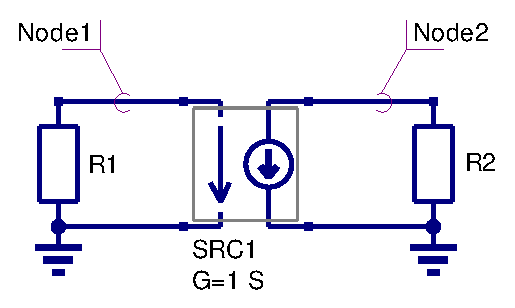
\includegraphics[width=7cm]{MNAnoise1}
\end{center}
\caption{simple non-reciprocal network}
\label{fig:mna_noise1}
\end{figure}
\FloatBarrier

Because of the controlled current source, the circuit is not
reciprocal. We want to know the noise voltage at node 2. Yes,
this is very easy to calculate, because it is a simple example,
but we want to use the algorithm described above.\\
We could solve the equations
\begin{equation}
\begin{bmatrix}
1/R_1 & 0\\
  G   & 1/R_2
\end{bmatrix}
\cdot
\begin{bmatrix}
Z_{11}\\
Z_{21}
\end{bmatrix}
=
\begin{bmatrix}
-1\\
0
\end{bmatrix}
\end{equation}
and
\begin{equation}
\begin{bmatrix}
1/R_1 & 0\\
  G   & 1/R_2
\end{bmatrix}
\cdot
\begin{bmatrix}
Z_{12}\\
Z_{22}
\end{bmatrix}
=
\begin{bmatrix}
0\\
-1
\end{bmatrix}
\end{equation}
So, we must solve the MNA matrix two times: First to get the
transimpedance from node 1 to node 2 (i.e. $Z_{21}$) and
second to get the transimpedance from node 2 to node 2 (i.e.
$Z_{22}$). But why solving it two times, if we only want to
know one voltage ? With every step we get transimpedances
that we do not need. Is there no more effective way ?

\addvspace{12pt}

Fortunately, we remember Tellegen's Theorem: A network and
its adjoint network are reciprocal to each other. That is,
we have to transpose the MNA matrix and the new matrix is
the one of the reciprocal network. Let's check it out:

\begin{equation}
[A]^T\cdot [x] =
\begin{bmatrix}
1/R_1 & G\\
  0   & 1/R_2
\end{bmatrix}
\cdot
\begin{bmatrix}
U_1\\
U_2
\end{bmatrix}
=
\begin{bmatrix}
0\\
0
\end{bmatrix}
\end{equation}

\begin{figure}[ht]
\begin{center}
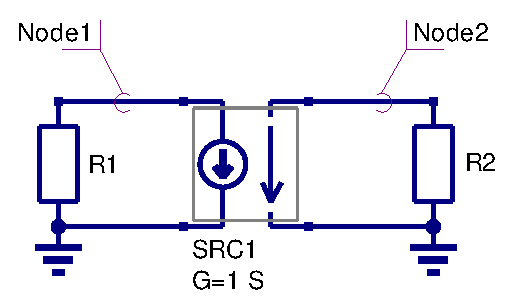
\includegraphics[width=7cm]{MNAnoise2}
\end{center}
\caption{simple network to compare with adjoint network}
\label{fig:mna_noise2}
\end{figure}
\FloatBarrier

Compare the transposed matrix with the reciprocal network
in figure \ref{fig:mna_noise2}. It is true! But now we
have:
\begin{equation}
\begin{bmatrix}
1/R_1 & G\\
  0   & 1/R_2
\end{bmatrix}
\cdot
\begin{bmatrix}
Z_{12,reciprocal}\\
Z_{22,reciprocal}
\end{bmatrix}
=
\begin{bmatrix}
1/R_1 & G\\
  0   & 1/R_2
\end{bmatrix}
\cdot
\begin{bmatrix}
Z_{21}\\
Z_{22}
\end{bmatrix}
=
\begin{bmatrix}
0\\
-1
\end{bmatrix}
\end{equation}
Because $Z_{21}$ of our original network equals $Z_{12}$ of
the reciprocal network, we get exactly what we need with one
step. So let us go on:
\begin{equation}
([A]^T)^{-1}\cdot
\begin{bmatrix}
  0\\
 -1
\end{bmatrix}
=
\begin{bmatrix}
R_1 & -G\cdot R_1\cdot R_2\\
  0 & R2
\end{bmatrix}
\cdot
\begin{bmatrix}
  0\\
 -1
\end{bmatrix}
=
\begin{bmatrix}
G\cdot R_1\cdot R_2\\
-R_2
\end{bmatrix}
=
\begin{bmatrix}
Z_{21}\\
Z_{22}
\end{bmatrix}
\end{equation}

Now, as we computed the transimpedances, we can
compute the noise voltages at node 2. As there is
no correlation, we get:

\begin{eqnarray}
<u_{node2}^2> & = & <u_{R1,node2}^2> + <u_{R2,node2}^2> \\
  & = & <i_{R1}^2>\cdot Z_{21}\cdot Z_{21}^* + <i_{R2}^2>\cdot Z_{22}\cdot Z_{22}^* \\
  & = & \frac{4\cdot k\cdot T\cdot \Delta f}{R_1} \cdot (G\cdot R_1\cdot R_2)^2 +
        \frac{4\cdot k\cdot T\cdot \Delta f}{R_2} \cdot (-R_2)^2 \\
  & = & 4\cdot k\cdot T\cdot \Delta f\cdot \left( R_1\cdot (G\cdot R_2)^2 + R_2 \right)
\end{eqnarray}

That's it. Yes, you knew it before, but now you also understand
the universal algorithm.



\section{Noise Current Correlation Matrix}
%\addcontentsline{toc}{section}{Noise Current Correlation Matrix}

This section describes the noise current correlation matrices of noisy
components.  The equations are built for RMS noise currents with
$1\hertz$ bandwidth.

\addvspace{12pt}

Resistor with resistance $R$ and temperature $T$:
\begin{equation}
(\underline{C}_Y) = \frac{4\cdot k\cdot T}{R} \cdot
\begin{pmatrix}
 1 & -1 \\
-1 &  1 \\
\end{pmatrix}
\end{equation}

Noise current source with a current power spectral density of $cPSD$:
\begin{equation}
(\underline{C}_Y) = cPSD \cdot
\begin{pmatrix}
 1 & -1 \\
-1 &  1 \\
\end{pmatrix}
\end{equation}

A noise voltage source (voltage power spectral density $vPSD$)
cannot be modeled with the noise current
matrix. That is why one has to use a noise current source
(current power spectral density $cPSD$) connected to a gyrator
(transimpedance $R$) satisfying the equation
\begin{equation}
vPSD = cPSD \cdot R
\end{equation}
Figure \ref{fig:Unoise} shows an example.

\begin{figure}[ht]
\begin{center}
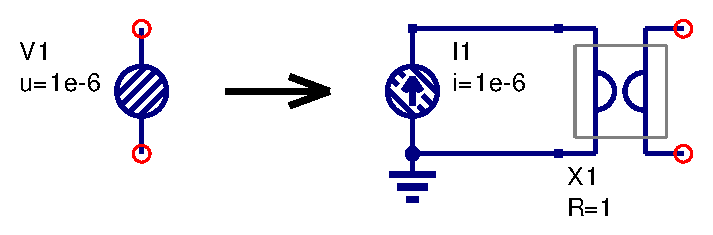
\includegraphics[width=9cm]{Unoise}
\end{center}
\caption{noise voltage source (left-hand side) and its equivalent circuit (right-hand side)}
\label{fig:Unoise}
\end{figure}
\FloatBarrier


Attenuator with (power) attenuation $L$, reference impedance $Z_{ref}$
and temperature $T$:
\begin{equation}
(\underline{C}_Y) = 4\cdot k\cdot T\cdot \text{Re}\left(\underline{Y}\right)
 = \frac{4\cdot k\cdot T}{Z_{ref}\cdot (L-1)} \cdot
\begin{pmatrix}
 L+1            & -2\cdot\sqrt{L} \\
-2\cdot\sqrt{L} &  L+1 \\
\end{pmatrix}
\end{equation}

Isolator with reference impedance $Z_1$ (input) and $Z_2$ (output) and
temperature $T$:
\begin{equation}
(\underline{C}_Y) = 4\cdot k\cdot T\cdot
\begin{pmatrix}
 1/Z_1                 & 0 \\
-2/\sqrt{Z_1\cdot Z_2} &  1/Z_2 \\
\end{pmatrix}
\end{equation}

Diode (for details on the parameters see section \ref{sec:nw_diode}):
\begin{equation}
(\underline{C}_Y)
 = 2\cdot e\cdot K\cdot \left(I_{d} + 2\cdot I_{S}\right)\cdot
\begin{pmatrix}
   1 & -1\\
  -1 &  1\\
\end{pmatrix}\\
\end{equation}
